% !TeX program = pdflatex
% =============================================================================
% Folien: Freier Fall und senkrechter Wurf
% Kantonsschule KFR, 4. Klasse, 1. HS, Mechanik
%
% Baut direkt auf ../bewegungsgleichungen/bewegungsgleichungen-wiederholung-
% folien.tex auf: gleiches Layout (Variante E "Petrol modern"), gleiche
% Schreibweise (s, s_0, v_0, t_0, t-t_0), gleicher Farbcode. Der freie Fall
% wird nicht neu hergeleitet, sondern als Spezialfall der vier bekannten
% Bewegungsgleichungen mit a = -g eingeführt.
%
% Konvention wie in arbeitsblaetter/.../freier-fall/freier-fall-arbeitsblatt.tex:
% nach oben positiv, also a = -g, g = 9.81 m/s^2, Luftwiderstand
% vernachlässigt. Das Arbeitsblatt schreibt den Ort als x, die Folien als s
% (Anschluss an die Bewegungsgleichungsfolien); die Rückblickfolie weist
% darauf hin.
%
% Aufbau (nach jeder Erklärung eine Aufgabe mit Lösungsfolie):
%   Rückblick Bewegungsgleichungen
%   Hammer und Feder (Predict/Explain, Aufgabe 1)            LZ2
%   Erdbeschleunigung g und Vorzeichen a = -g (Aufgabe 2)      LZ1, Lernschw. 5
%   Freier Fall aus der Ruhe, Fallzeit (Aufgabe 3)             LZ3
%   Senkrechter Wurf, Umkehrpunkt (Aufgabe 4, ConcepTest)      LZ5, Lernschw. 2
%   Steigzeit, maximale Höhe, Flugzeit (Aufgabe 5)             LZ4
%   Diagramme mit Steigung und Fläche (Aufgabe 6)              LZ6
%
% Farbcode: s_0 blau, v_0 orange, a bzw. g violett, t-t_0 grün (petrol).
% =============================================================================
\documentclass[14pt,aspectratio=169]{beamer}

\usepackage[T1]{fontenc}
\usepackage[utf8]{inputenc}
\usepackage[ngerman]{babel}
\usepackage{amsmath}
\usepackage{siunitx}
% Hausstil: zusammengesetzte Einheiten immer als echter Bruch (\frac), nicht
% als Inline-Schrägstrich oder \tfrac -- gilt global für jedes \si/\SI.
\sisetup{per-mode=fraction,fraction-command=\frac}
\usepackage{tikz}
\usetikzlibrary{decorations.pathreplacing,arrows.meta,calc}
\usepackage{physics}
\usepackage{circuitikz}
\usepackage{booktabs}
\usepackage[most]{tcolorbox}
\usepackage{cancel}
\renewcommand{\CancelColor}{\color{orangeakzent}}
\usepackage{graphicx}
\usepackage[default]{sourcesanspro}
% Schullogo liegt in institutionen/KFR/kfr_logo.png (fünf Ebenen höher),
% Bilder des Arbeitsblatts unter arbeitsblaetter/... relativ dazu.
\graphicspath{{../../../../../}}

% --- Layout "Petrol modern" (Variante E aus folien/logo-varianten/) ---------
\usetheme{default}
\usefonttheme{professionalfonts}
\setbeamertemplate{navigation symbols}{}
\setbeamertemplate{sidebar}{}
\setbeamertemplate{headline}{}
\beamertemplatenavigationsymbolsempty

\definecolor{kfrgrau}{RGB}{90,90,90}
\definecolor{petrol}{HTML}{14555F}
\definecolor{hellpetrol}{HTML}{E4F0F1}
\definecolor{orangeakzent}{HTML}{E07A1F}

\setbeamercolor{normal text}{fg=black,bg=white}
\setbeamercolor{structure}{fg=petrol}
\setbeamercolor{title}{fg=petrol,bg=white}
\setbeamercolor{frametitle}{fg=petrol,bg=white}
\setbeamercolor{footline}{fg=kfrgrau,bg=white}
\setbeamercolor{page number in head/foot}{fg=kfrgrau}
\setbeamercolor{itemize item}{fg=petrol}
\setbeamercolor{itemize subitem}{fg=petrol}

\setbeamerfont{frametitle}{size=\Large,series=\bfseries}
\setbeamerfont{title}{size=\LARGE,series=\bfseries}
\setbeamerfont{itemize item}{size=\normalsize}

\setbeamertemplate{itemize item}{\textbullet}
\setbeamertemplate{itemize subitem}{--}

\setbeamertemplate{frametitle}{%
  \nointerlineskip
  \vspace*{0.15cm}%
  \begin{beamercolorbox}[wd=\paperwidth,leftskip=1cm,rightskip=3.2cm plus 1fil]{frametitle}
    \hyphenpenalty=10000
    {\scriptsize\scshape\color{orangeakzent}\insertshorttitle\par}\vspace{-0.15em}
    {\usebeamerfont{frametitle}\insertframetitle\par}
    \vspace{0.05em}
    {\color{orangeakzent}\rule{2.4cm}{2pt}}\par\vspace{-0.9em}
  \end{beamercolorbox}%
  \begin{tikzpicture}[remember picture,overlay]
    \node[anchor=north east,inner sep=0pt] at ([xshift=-0.5cm,yshift=-0.4cm]current page.north east)
      {
\includegraphics[height=0.6cm]{kfr_logo}};
  \end{tikzpicture}%
}

\setbeamertemplate{footline}{%
  \begin{beamercolorbox}[wd=\paperwidth,ht=0.35cm,dp=0.15cm,leftskip=1cm,rightskip=1cm]{footline}
    \scriptsize\insertshorttitle\hfill\insertframenumber\,/\,\inserttotalframenumber
  \end{beamercolorbox}
}

% --- Farben wie in den Arbeitsblättern ---------------------------------------
\definecolor{titleblue}{HTML}{183A6B}
\definecolor{lightblue}{HTML}{EAF4FB}
\definecolor{accentorange}{HTML}{D9720C}
\definecolor{lightorange}{HTML}{FCEEE0}
\definecolor{accentpurple}{HTML}{7B2D8E}
\definecolor{lightpurple}{HTML}{F3EAF7}
\definecolor{groupteal}{HTML}{1B7F72}
\definecolor{lightgroupteal}{HTML}{E8F5F3}
\definecolor{theoriegreen}{HTML}{2E7D32}
\definecolor{lighttheoriegreen}{HTML}{EDF7EE}

% --- Boxen: Merksatz (grün, wie theoriebox) und Aufgabe (Petrol, Layoutfarbe) -
\newtcolorbox{merkbox}[1][Merke]{enhanced,colback=lighttheoriegreen,
  colframe=theoriegreen,fonttitle=\bfseries\small,title={#1},boxrule=0.8pt,
  arc=2pt,left=4pt,right=4pt,top=2pt,bottom=2pt}
\newtcolorbox{aufgabebox}[1][Aufgabe]{enhanced,colback=hellpetrol,
  colframe=petrol,fonttitle=\bfseries\small,title={#1},boxrule=0.8pt,
  arc=2pt,left=4pt,right=4pt,top=2pt,bottom=2pt}

% --- Farbige Symbole (Farbcode siehe Dateikopf) ------------------------------
\newcommand{\Szero}{\textcolor{titleblue}{s_0}}
\newcommand{\Vzero}{\textcolor{accentorange}{v_0}}
\newcommand{\Tzero}{\textcolor{groupteal}{t_0}}
\newcommand{\Acol}{\textcolor{accentpurple}{a}}
\newcommand{\Gcol}{\textcolor{accentpurple}{g}}
\newcommand{\Tdiff}{\textcolor{groupteal}{(t-t_0)}}

% --- Einheiten sichtbar mitrechnen (wie in den Bewegungsgleichungsfolien) ----
% \ein{m}: Einheit als aufrechtes Zeichen, \kue{s}: gekürzte Einheit (orange
% durchgestrichen), \Eh{...}: graue Randnotiz, was mit den Einheiten passiert.
\newcommand{\ein}[1]{\mathrm{#1}}
\newcommand{\kue}[1]{\cancel{\mathrm{#1}}}
\newcommand{\Eh}[1]{\text{\footnotesize\color{kfrgrau}#1}}

\title{Freier Fall}
\subtitle{Die Bewegungsgleichungen mit $a=-g$}
\author{}
\institute{Kantonsschule KFR, 4. Klasse}
\date{\today}

\begin{document}

% --- Titelfolie --------------------------------------------------------------
\begin{frame}[plain]
  \begin{tikzpicture}[remember picture,overlay]
    \fill[hellpetrol] ([xshift=-5.6cm]current page.north east) rectangle (current page.south east);
    \node[inner sep=0pt] at ([xshift=-2.8cm]current page.east)
      {
\includegraphics[width=4.4cm]{kfr_logo}};
    \fill[orangeakzent] ([xshift=-5.6cm]current page.north east) rectangle ++(0.12cm,-\paperheight);
  \end{tikzpicture}
  \begin{minipage}{0.66\textwidth}
    {\small\scshape\color{orangeakzent}Physik \textperiodcentered{} 4. Klasse\par}
    \vspace{0.4em}
    {\usebeamerfont{title}\usebeamercolor[fg]{title}\inserttitle\par}
    \vspace{0.3em}
    {\color{orangeakzent}\rule{2.4cm}{2pt}\par}
    \vspace{0.5em}
    {\large\insertsubtitle\par}
    \vspace{1em}
    {\small\color{kfrgrau}\insertdate\par}
  \end{minipage}
\end{frame}

\begin{frame}{Fahrplan}
  \small
  \begin{enumerate}
    \setlength{\itemsep}{0pt}
    \item \textbf{Rückblick:} die vier Bewegungsgleichungen
    \item \textbf{Hammer und Feder:} Fallen schwere Dinge schneller?
    \item \textbf{Die Erdbeschleunigung $g$} und ihr Vorzeichen
    \item \textbf{Freier Fall aus der Ruhe:} Fallstrecke und Fallzeit
    \item \textbf{Wurf nach oben:} Umkehrpunkt, Steigzeit, maximale Höhe
    \item \textbf{Diagramme:} Steigung und Fläche beim Wurf
  \end{enumerate}
  \vspace{0.2em}
  \begin{merkbox}[Die gute Nachricht]
    Keine neuen Gleichungen: Der freie Fall ist eine gleichmässig
    beschleunigte Bewegung mit $a=-g$.
  \end{merkbox}
\end{frame}

% =============================================================================
% Rückblick
% =============================================================================
\begin{frame}{Rückblick: Bewegungsgleichungen}
  \small
  \centering
  \begin{tabular}{lll}
    \toprule
    & \textbf{Gleichung} & \textbf{Wann?} \\
    \midrule
    1 & $s(t)=s_0+v\,(t-t_0)$ & $v$ konstant ($a=0$) \\[0.2em]
    2 & $v(t)=v_0+a\,(t-t_0)$ & $a$ konstant, Ort egal \\[0.2em]
    3 & $s(t)=s_0+v_0(t-t_0)+\tfrac12\,a\,(t-t_0)^2$ & $a$ konstant, Ort und Zeit \\[0.2em]
    4 & $v^2=v_0^2+2\,a\,\Delta s$ & $a$ konstant, Zeit egal \\
    \bottomrule
  \end{tabular}

  \vspace{0.6em}
  \begin{merkbox}[Erinnerung]
    \centering
    $t-t_0=\Delta t$ \ (Zeit seit dem Start) \qquad
    $s-s_0=\Delta s$ \qquad
    $v-v_0=\Delta v$
  \end{merkbox}
  \footnotesize
  Beim freien Fall ist $s$ die Höhe. Auf dem Arbeitsblatt heisst sie $x$,
  gemeint ist dasselbe.
\end{frame}

% =============================================================================
% Hammer und Feder (Predict, dann Explain)
% =============================================================================
\begin{frame}{Aufgabe 1: Hammer und Feder}
  \begin{columns}[c]
    \begin{column}{0.45\textwidth}
      \centering
      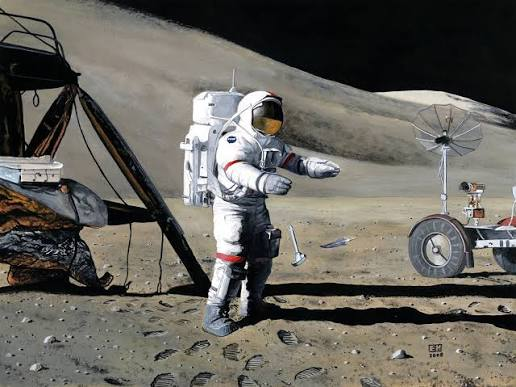
\includegraphics[width=\linewidth]{arbeitsblaetter/4-klasse/1-hs/mechanik/freier-fall/Bilder/Apollo_15.jpg}\\[0.2em]
      {\tiny Illustration: Apollo 15, David Scott, 1971}
    \end{column}
    \begin{column}{0.53\textwidth}
      \begin{aufgabebox}[Aufgabe 1: Zuerst vorhersagen!]
        \small
        Ein Astronaut lässt auf dem Mond einen Hammer und eine Feder
        gleichzeitig aus derselben Höhe los. Auf dem Mond gibt es keine
        Luft.
        \begin{enumerate}
          \item[a)] Was landet zuerst? Notiere zuerst deine Vorhersage
            mit Begründung.
          \item[b)] Was würde auf der Erde passieren?
        \end{enumerate}
      \end{aufgabebox}
    \end{column}
  \end{columns}
\end{frame}

\begin{frame}{Aufgabe 1: Auflösung}
  \small
  a) Hammer und Feder landen auf dem Mond \textbf{genau gleichzeitig}.
  Das ist gefilmt (NASA, Apollo 15).

  \vspace{0.3em}
  b) Auf der Erde fällt der Hammer schneller. Grund ist aber nicht die
  Masse, sondern der \textbf{Luftwiderstand}: Er bremst die leichte,
  grosse Feder stark, den Hammer kaum.

  \vspace{0.4em}
  \begin{merkbox}[Modell: freier Fall]
    Ohne Luftwiderstand fallen \textbf{alle Körper gleich}, unabhängig
    von ihrer Masse. Sie haben alle dieselbe Beschleunigung, die
    \textbf{Fallbeschleunigung} $g$. Mit diesem Modell rechnen wir ab
    jetzt.
  \end{merkbox}
  \footnotesize
  Galileo Galilei kam schon um 1600 zu diesem Schluss, mit Kugeln auf einer
  schiefen Ebene.
\end{frame}

% =============================================================================
% Erdbeschleunigung g und Vorzeichen
% =============================================================================
\begin{frame}{Die Erdbeschleunigung $g$}
  \small
  \begin{columns}[T]
    \begin{column}{0.5\textwidth}
      Nahe der Erdoberfläche gilt:
      \[
        g\approx\SI{9.81}{\meter\per\second\squared}
      \]
      Das heisst: Jede Sekunde wird ein fallender Körper um
      $\SI{9.81}{\meter\per\second}$ (rund $\SI{35}{\kilo\meter\per\hour}$)
      schneller.

      \vspace{0.4em}
      Auf dem Mond ist
      $g_{\text{Mond}}\approx\SI{1.62}{\meter\per\second\squared}$, nur
      etwa ein Sechstel.
    \end{column}
    \begin{column}{0.46\textwidth}
      \centering
      \begin{tabular}{rrr}
        \toprule
        $t$ in s & Geschw. in $\si{\meter\per\second}$ & in $\si{\kilo\meter\per\hour}$ \\
        \midrule
        0 & 0\phantom{.00} & 0 \\
        1 & 9.81 & 35 \\
        2 & 19.62 & 71 \\
        3 & 29.43 & 106 \\
        \bottomrule
      \end{tabular}\\[0.4em]
      \footnotesize Freier Fall aus der Ruhe
    \end{column}
  \end{columns}
\end{frame}

\begin{frame}{Einheiten beim freien Fall}
  \small
  Wie bei den Bewegungsgleichungen rechnen wir die Einheiten immer mit.
  Diese vier Fälle kommen beim freien Fall ständig vor:
  \begin{align*}
    \SI{9.81}{\meter\per\second\squared}\cdot\SI{1}{\second}
      &= 9.81\cdot\frac{\ein{m}}{\ein{s}\cdot\kue{s}}\cdot\kue{s}
       = \SI{9.81}{\meter\per\second}
      && \Eh{m/s$^2$ mal s ergibt m/s}\\
    \tfrac12\cdot\SI{9.81}{\meter\per\second\squared}\cdot\SI{4}{\second\squared}
      &= \tfrac12\cdot9.81\cdot4\cdot\frac{\ein{m}}{\kue{\ein{s}^2}}\cdot\kue{\ein{s}^2}
       = \SI{19.62}{\meter}
      && \Eh{m/s$^2$ mal s$^2$ ergibt m}\\
    \frac{\SI{18}{\meter}}{\SI{9.81}{\meter\per\second\squared}}
      &= \frac{18}{9.81}\cdot\kue{m}\cdot\frac{\ein{s}^2}{\kue{m}}
       \approx \SI{1.83}{\second\squared}
      && \Eh{durch m/s$^2$ teilen heisst mal s$^2$/m}\\
    \sqrt{\SI{1.83}{\second\squared}}
      &= \sqrt{1.83}\cdot\sqrt{\ein{s}^2}\approx\SI{1.35}{\second}
      && \Eh{die Wurzel wirkt auf Zahl und Einheit}
  \end{align*}
\end{frame}

\begin{frame}{Vorzeichen: $g$ zeigt nach unten}
  \begin{columns}[T]
    \begin{column}{0.3\textwidth}
      \centering
      \begin{tikzpicture}[scale=0.8]
        \draw[->,thick] (0,-0.2) -- (0,4.2) node[above] {\small $s$};
        \node[left] at (0,4) {\scriptsize oben $+$};
        \draw (-0.12,0.5) -- (0.12,0.5) node[right] {\scriptsize $0$};
        \fill[kfrgrau!30] (-1.4,-0.2) rectangle (1.4,0);
        \filldraw[accentorange] (1.1,2.6) circle (0.2);
        \draw[-{Latex[length=2.5mm]},very thick,accentpurple] (1.1,2.3) -- (1.1,1.0)
          node[right,midway] {\small $g$};
      \end{tikzpicture}
    \end{column}
    \begin{column}{0.68\textwidth}
      \small
      Wir legen fest: \textbf{nach oben ist positiv}. Die Fallbeschleunigung
      zeigt nach unten, also
      \[
        \Acol=-\Gcol \qquad (g=\SI{9.81}{\meter\per\second\squared}\text{ ist der Betrag})
      \]
      Eingesetzt in die Bewegungsgleichungen:
      \begin{align*}
        v(t) &= \Vzero-\Gcol\,\Tdiff\\
        s(t) &= \Szero+\Vzero\Tdiff-\tfrac12\,\Gcol\Tdiff^2\\
        v^2  &= \Vzero^2-2\,\Gcol\,\Delta s
      \end{align*}
    \end{column}
  \end{columns}
\end{frame}

\begin{frame}{Aufgabe 2: Vorzeichen}
  \begin{aufgabebox}[Aufgabe 2]
    \small
    Ein Ball wird senkrecht nach oben geworfen. Nach oben ist positiv.
    Welches Vorzeichen haben $v$ und $a$ in den drei Momenten?
    \vspace{0.3em}

    \centering
    \begin{tabular}{lcc}
      \toprule
      & $v$ & $a$ \\
      \midrule
      A: Der Ball steigt noch nach oben. & ? & ? \\
      B: Der Ball ist am höchsten Punkt. & ? & ? \\
      C: Der Ball fällt wieder nach unten. & ? & ? \\
      \bottomrule
    \end{tabular}
  \end{aufgabebox}
\end{frame}

\begin{frame}{Aufgabe 2: Lösung}
  \small
  \centering
  \begin{tabular}{lcc}
    \toprule
    & $v$ & $a$ \\
    \midrule
    A: Der Ball steigt noch nach oben. & $+$ & $-g$ \\
    B: Der Ball ist am höchsten Punkt. & $0$ & $-g$ \\
    C: Der Ball fällt wieder nach unten. & $-$ & $-g$ \\
    \bottomrule
  \end{tabular}

  \vspace{0.6em}
  \raggedright
  \begin{merkbox}[Merke]
    Das Vorzeichen von $v$ sagt, \textbf{wohin} sich der Ball bewegt. Die
    Beschleunigung ist während des ganzen Flugs dieselbe: $a=-g$.
  \end{merkbox}
  \footnotesize
  In A haben $v$ und $a$ verschiedene Vorzeichen: Der Ball wird
  langsamer. In C haben beide dasselbe Vorzeichen: Er wird schneller.
\end{frame}

% =============================================================================
% Freier Fall aus der Ruhe
% =============================================================================
\begin{frame}{Freier Fall aus der Ruhe}
  \begin{columns}[T]
    \begin{column}{0.62\textwidth}
      \small
      Loslassen: $\Vzero=0$. Stoppuhr und Nullpunkt beim Start:
      $\Tzero=0$, $\Szero=0$.
      \begin{align*}
        v(t) &= 0-g\,(t-0) = -g\,t\\
        s(t) &= 0+0-\tfrac12\,g\,(t-0)^2 = -\tfrac12\,g\,t^2
      \end{align*}
      Das Minus heisst: unter dem Start, nach unten. Als Beträge:
      \begin{merkbox}[Freier Fall aus der Ruhe]
        \centering
        Fallstrecke $h=\tfrac12\,g\,t^2$ \qquad Geschw. $|v|=g\,t$
      \end{merkbox}
    \end{column}
    \begin{column}{0.34\textwidth}
      \centering
      \begin{tikzpicture}[scale=0.8]
        \draw[->,thick] (0,-3.6) -- (0,0.5) node[above] {\scriptsize $s$ in m};
        \foreach \t/\h/\l in {0/0/0,1/4.9/-4.9,2/19.6/-19.6,3/44.1/-44.1} {
          \filldraw[accentorange] (0.6,-\h*0.075) circle (0.13);
          \draw[gray] (-0.08,-\h*0.075) -- (0.08,-\h*0.075);
          \node[left] at (-0.1,-\h*0.075) {\scriptsize $\l$};
          \node[right] at (0.8,-\h*0.075) {\scriptsize $t=\SI{\t}{\second}$};
        }
      \end{tikzpicture}\\[0.2em]
      \footnotesize Jede Sekunde ein Foto: Die Abstände wachsen.
      Das ist $s=\tfrac12\,a\,t^2$ aus dem Stand mit $a=g$.
    \end{column}
  \end{columns}
\end{frame}

\begin{frame}{Fallzeit aus der Fallhöhe}
  \small
  Oft ist die Höhe $h$ gegeben und die Fallzeit $t$ gesucht. Wir lösen
  $h=\tfrac12\,g\,t^2$ nach $t$ auf:
  \begin{align*}
    h &= \tfrac12\,g\,t^2 && \text{\footnotesize mal 2}\\
    2h &= g\,t^2 && \text{\footnotesize durch } g\\
    \frac{2h}{g} &= t^2 && \text{\footnotesize Wurzel ziehen}\\
    t &= \sqrt{\frac{2h}{g}}
  \end{align*}
  \footnotesize
  Die negative Wurzel verwerfen wir: Die Zeit seit dem Loslassen kann nicht
  negativ sein.

  Einheitenkontrolle:
  $\sqrt{\dfrac{\ein{m}}{\ein{m}/\ein{s}^2}}
   =\sqrt{\kue{m}\cdot\dfrac{\ein{s}^2}{\kue{m}}}
   =\sqrt{\ein{s}^2}=\ein{s}$, also eine Zeit.
\end{frame}

\begin{frame}{Aufgabe 3: Blumentopf vom Balkon}
  \begin{aufgabebox}[Aufgabe 3]
    \small
    Vom Balkon im 3. Stock fällt ein Blumentopf aus $h=\SI{9.0}{\meter}$
    Höhe auf den Boden. Luftwiderstand vernachlässigen,
    $g=\SI{9.81}{\meter\per\second\squared}$.
    \begin{enumerate}
      \item[a)] Wie lange dauert der Fall?
      \item[b)] Wie schnell ist der Topf beim Aufprall? Gib das Resultat in
        $\si{\meter\per\second}$ und $\si{\kilo\meter\per\hour}$ an.
      \item[c)] Kontrolliere b) mit Gleichung 4 ($v^2=v_0^2+2\,a\,\Delta s$).
        Achte auf die Vorzeichen von $a$ und $\Delta s$.
    \end{enumerate}
  \end{aufgabebox}
\end{frame}

\begin{frame}{Aufgabe 3: Lösung a)}
  \small
  a) Fallzeit:
  \begin{align*}
    t &= \sqrt{\frac{2h}{g}}
       = \sqrt{\frac{2\cdot\SI{9.0}{\meter}}{\SI{9.81}{\meter\per\second\squared}}}
      && \Eh{Werte mit Einheiten einsetzen}\\
      &= \sqrt{\frac{\SI{18.0}{\meter}}{\SI{9.81}{\meter\per\second\squared}}}
       = \sqrt{\frac{18.0}{9.81}\cdot\kue{m}\cdot\frac{\ein{s}^2}{\kue{m}}}
      && \Eh{durch m/s$^2$ teilen heisst mal s$^2$/m}\\
      &= \sqrt{\SI{1.835}{\second\squared}}
       = \sqrt{1.835}\cdot\sqrt{\ein{s}^2}
      && \Eh{Wurzel aus Zahl und aus Einheit}\\
      &\approx \SI{1.35}{\second}
      && \Eh{$\sqrt{\ein{s}^2}=\ein{s}$}
  \end{align*}
\end{frame}

\begin{frame}{Aufgabe 3: Lösung b)}
  \small
  b) Aufprallgeschwindigkeit (mit dem ungerundeten $t=\SI{1.355}{\second}$):
  \begin{align*}
    |v| &= g\,t
         = \SI{9.81}{\meter\per\second\squared}\cdot\SI{1.355}{\second}
      && \Eh{Werte mit Einheiten einsetzen}\\
        &= 9.81\cdot1.355\cdot\frac{\ein{m}}{\ein{s}\cdot\kue{s}}\cdot\kue{s}
      && \Eh{ein s kürzt sich, es bleibt m/s}\\
        &\approx \SI{13.3}{\meter\per\second}\\
        &= 13.3\cdot3.6\,\si{\kilo\meter\per\hour}
         \approx \SI{48}{\kilo\meter\per\hour}
      && \Eh{m/s mal 3.6 ergibt km/h}
  \end{align*}
\end{frame}

\begin{frame}{Aufgabe 3: Lösung c)}
  \small
  c) Nach oben positiv: Der Topf bewegt sich nach unten, also
  $\Delta s=-\SI{9.0}{\meter}$, und $a=-g=-\SI{9.81}{\meter\per\second\squared}$.
  \begin{align*}
    v^2 &= v_0^2+2\,a\,\Delta s
         = 0+2\cdot\left(-\SI{9.81}{\meter\per\second\squared}\right)\cdot\left(-\SI{9.0}{\meter}\right)
      && \Eh{Minus mal Minus gibt Plus}\\
        &= 2\cdot9.81\cdot9.0\cdot\frac{\ein{m}}{\ein{s}^2}\cdot\ein{m}
         = \SI{176.6}{\meter\squared\per\second\squared}
      && \Eh{m mal m ergibt m$^2$}\\
    v &= -\sqrt{\SI{176.6}{\meter\squared\per\second\squared}}
       = -\sqrt{176.6}\cdot\sqrt{\frac{\ein{m}^2}{\ein{s}^2}}
      && \Eh{Wurzel aus Zahl und aus Einheit}\\
      &\approx-\SI{13.3}{\meter\per\second}
      && \Eh{$\sqrt{\ein{m}^2/\ein{s}^2}=\ein{m}/\ein{s}$}
  \end{align*}
  Wir nehmen die \textbf{negative} Wurzel, weil sich der Topf nach unten
  bewegt. Der Betrag stimmt mit b) überein.
\end{frame}

% =============================================================================
% Senkrechter Wurf nach oben, Umkehrpunkt
% =============================================================================
\begin{frame}{Senkrechter Wurf nach oben}
  \begin{columns}[T]
    \begin{column}{0.55\textwidth}
      \small
      Jetzt ist $\Vzero>0$ (nach oben). Die Beschleunigung bleibt
      $a=-g$. Mit $\Szero=0$ und $\Tzero=0$:
      \begin{merkbox}[Wurf nach oben]
        \centering
        $v(t)=\Vzero-g\,t$\\[0.3em]
        $s(t)=\Vzero\,t-\tfrac12\,g\,t^2$
      \end{merkbox}
      Der Ball wird beim Steigen jede Sekunde um
      $\SI{9.81}{\meter\per\second}$ langsamer, bis er kurz stillsteht.
      Danach fällt er und wird wieder schneller.
    \end{column}
    \begin{column}{0.41\textwidth}
      \centering
      \begin{tikzpicture}[scale=0.8]
        \draw[->] (-0.2,0) -- (4.6,0) node[right] {$t$};
        \draw[->] (0,-2.2) -- (0,2.5) node[above] {$v$};
        \draw[very thick,accentorange] (0,2) -- (4,-2);
        \node[left] at (0,2) {$\Vzero$};
        \filldraw (2,0) circle (2pt);
        \node[below left] at (2,0) {\scriptsize $t_S$};
        % Labels neben die Gerade y = 2 - x setzen, nicht darauf:
        % "steigt" oberhalb, "fällt" unterhalb der Linie.
        \node[accentorange,above right=1pt] at (1,1) {\scriptsize steigt};
        \node[accentorange,below left=1pt] at (3,-1) {\scriptsize fällt};
      \end{tikzpicture}\\[0.2em]
      \footnotesize $v$ nimmt gleichmässig ab: Gerade mit Steigung $-g$.
    \end{column}
  \end{columns}
\end{frame}

\begin{frame}{Aufgabe 4: Der höchste Punkt}
  \begin{aufgabebox}[Aufgabe 4: Abstimmung]
    \small
    Ein Ball wird senkrecht nach oben geworfen. Was gilt im höchsten Punkt
    der Flugbahn? Stimme zuerst allein ab, diskutiere dann mit deiner
    Nachbarin oder deinem Nachbarn und stimme nochmals ab.
    \begin{enumerate}
      \item[A)] $v=0$ und $a=0$
      \item[B)] $v=0$ und $a=-g$
      \item[C)] $v=0$ und $a=+g$
      \item[D)] $v=0$, und $a$ wechselt dort von $-g$ zu $+g$
    \end{enumerate}
  \end{aufgabebox}
\end{frame}

\begin{frame}{Aufgabe 4: Lösung}
  \begin{columns}[T]
    \begin{column}{0.55\textwidth}
      \small
      Richtig ist \textbf{B}: $v=0$, aber $a=-g$.

      \vspace{0.3em}
      $a$ sagt nicht, wie schnell der Ball ist, sondern wie sich $v$
      \textbf{ändert}. Im höchsten Punkt ändert sich $v$ weiter: von
      positiv (nach oben) zu negativ (nach unten).

      \vspace{0.3em}
      Wäre dort $a=0$, bliebe $v=0$ für immer: Der Ball bliebe in der Luft
      stehen.
    \end{column}
    \begin{column}{0.41\textwidth}
      \centering
      \begin{tikzpicture}[scale=0.8]
        \draw[->] (-0.2,0) -- (4.6,0) node[right] {$t$};
        \draw[->] (0,-2.2) -- (0,2.5) node[above] {$v$};
        \draw[very thick,accentorange] (0,2) -- (4,-2);
        \filldraw (2,0) circle (2pt);
        \node[below left] at (2,0) {\scriptsize $t_S$};
        \draw[thick,groupteal] (2,0) -- (3,0);
        \draw[thick,accentpurple] (3,0) -- (3,-1);
        \node[right,accentpurple,align=left] at (3,-0.5) {\scriptsize Steigung\\[-0.3em]\scriptsize $=-g$};
      \end{tikzpicture}\\[0.2em]
      \footnotesize Bei $t_S$ ist $v=0$, die Steigung ist aber dieselbe
      wie überall.
    \end{column}
  \end{columns}
\end{frame}

% =============================================================================
% Steigzeit, maximale Höhe, Flugzeit
% =============================================================================
\begin{frame}{Steigzeit und maximale Höhe}
  \small
  Im höchsten Punkt gilt $v=0$. Das setzen wir in bekannte Gleichungen ein.
  \begin{columns}[T]
    \begin{column}{0.46\textwidth}
      \textbf{Steigzeit $t_S$} (Gl.~2):
      \begin{align*}
        0 &= v_0-g\,t_S && \text{\footnotesize $+g\,t_S$}\\
        g\,t_S &= v_0 && \text{\footnotesize durch } g\\
        t_S &= \frac{v_0}{g}
      \end{align*}
    \end{column}
    \begin{column}{0.52\textwidth}
      \textbf{Maximale Höhe} (Gl.~4, $\Delta s=h_{\max}$):
      \begin{align*}
        0 &= v_0^2-2\,g\,h_{\max} && \text{\footnotesize $+2g\,h_{\max}$}\\
        2\,g\,h_{\max} &= v_0^2 && \text{\footnotesize durch } 2g\\
        h_{\max} &= \frac{v_0^2}{2g}
      \end{align*}
    \end{column}
  \end{columns}
  \begin{merkbox}[Flugzeit bis zurück auf Abwurfhöhe]
    Hinauf und hinunter dauern gleich lang (gleiches $g$): \
    $T=2\,t_S=2\,v_0/g$.
  \end{merkbox}
\end{frame}

\begin{frame}{Aufgabe 5: Tennisball nach oben}
  \begin{aufgabebox}[Aufgabe 5]
    \small
    Du wirfst einen Tennisball mit $v_0=\SI{12}{\meter\per\second}$
    senkrecht nach oben. Nach oben ist positiv, Abwurfhöhe ist $s_0=0$.
    \begin{enumerate}
      \item[a)] Nach welcher Zeit ist der Ball am höchsten Punkt?
      \item[b)] Wie hoch fliegt er über die Abwurfhöhe?
      \item[c)] Nach welcher Zeit ist er wieder auf Abwurfhöhe?
      \item[d)] Wo ist der Ball nach $t=\SI{2}{\second}$, und wie schnell
        ist er? Fliegt er nach oben oder nach unten?
    \end{enumerate}
  \end{aufgabebox}
\end{frame}

\begin{frame}{Aufgabe 5: Lösung a) und c)}
  \small
  a) Steigzeit:
  \begin{align*}
    t_S &= \frac{v_0}{g}
         = \frac{\SI{12}{\meter\per\second}}{\SI{9.81}{\meter\per\second\squared}}
      && \Eh{Werte mit Einheiten einsetzen}\\
        &= \frac{12}{9.81}\cdot\frac{\ein{m}}{\ein{s}}\cdot\frac{\ein{s}\cdot\ein{s}}{\ein{m}}
      && \Eh{durch m/s$^2$ teilen heisst mal s$^2$/m}\\
        &= \frac{12}{9.81}\cdot\frac{\kue{m}\cdot\kue{s}\cdot\ein{s}}{\kue{s}\cdot\kue{m}}
         \approx\SI{1.223}{\second}\approx\SI{1.22}{\second}
      && \Eh{m und ein s kürzen sich, es bleibt s}
  \end{align*}
  c) Flugzeit, mit dem ungerundeten $t_S$ (sonst verdoppelt sich der
  Rundungsfehler):
  \[
    T=2\,t_S=2\cdot\SI{1.223}{\second}\approx\SI{2.45}{\second}
    \qquad\Eh{Zahl mal Zeit ergibt wieder eine Zeit}
  \]
\end{frame}

\begin{frame}{Aufgabe 5: Lösung b)}
  \small
  b) Maximale Höhe:
  \begin{align*}
    h_{\max} &= \frac{v_0^2}{2g}
       = \frac{\left(\SI{12}{\meter\per\second}\right)^2}{2\cdot\SI{9.81}{\meter\per\second\squared}}
      && \Eh{Werte mit Einheiten einsetzen}\\
      &= \frac{\SI{144}{\meter\squared\per\second\squared}}{\SI{19.62}{\meter\per\second\squared}}
      && \Eh{oben: Zahl und Einheit quadrieren}\\
      &= \frac{144}{19.62}\cdot\frac{\ein{m}^2}{\ein{s}^2}\cdot\frac{\ein{s}^2}{\ein{m}}
      && \Eh{durch m/s$^2$ teilen heisst mal s$^2$/m}\\
      &= \frac{144}{19.62}\cdot\frac{\ein{m}\cdot\kue{m}\cdot\kue{\ein{s}^2}}{\kue{\ein{s}^2}\cdot\kue{m}}
       \approx\SI{7.34}{\meter}
      && \Eh{s$^2$ und ein m kürzen sich, es bleibt m}
  \end{align*}
\end{frame}

\begin{frame}{Aufgabe 5: Lösung d), Teil 1}
  \small
  d) Ort nach $t=\SI{2}{\second}$. Das liegt nach $t_S$: Der Ball fällt
  schon wieder.
  \begin{align*}
    s &= v_0\,t-\tfrac12\,g\,t^2
       = \SI{12}{\meter\per\second}\cdot\SI{2}{\second}
        -\tfrac12\cdot\SI{9.81}{\meter\per\second\squared}\cdot(\SI{2}{\second})^2
      && \Eh{Werte mit Einheiten einsetzen}\\
      &= 12\cdot2\cdot\frac{\ein{m}}{\kue{s}}\cdot\kue{s}
        -\tfrac12\cdot9.81\cdot4\cdot\frac{\ein{m}}{\kue{\ein{s}^2}}\cdot\kue{\ein{s}^2}
      && \Eh{$(\SI{2}{\second})^2=\SI{4}{\second\squared}$, dann kürzen}\\
      &= \SI{24}{\meter}-\SI{19.62}{\meter}
      && \Eh{beide Terme in m}\\
      &\approx \SI{4.38}{\meter}
      && \Eh{gleiche Einheit: einfach subtrahieren}
  \end{align*}
  Der Ball ist $\SI{4.38}{\meter}$ über der Abwurfhöhe.
\end{frame}

\begin{frame}{Aufgabe 5: Lösung d), Teil 2}
  \small
  d) Geschwindigkeit nach $t=\SI{2}{\second}$:
  \begin{align*}
    v &= v_0-g\,t
       = \SI{12}{\meter\per\second}-\SI{9.81}{\meter\per\second\squared}\cdot\SI{2}{\second}
      && \Eh{Werte mit Einheiten einsetzen}\\
      &= \SI{12}{\meter\per\second}-9.81\cdot2\cdot\frac{\ein{m}}{\ein{s}\cdot\kue{s}}\cdot\kue{s}
      && \Eh{ein s kürzt sich, es bleibt m/s}\\
      &= \SI{12}{\meter\per\second}-\SI{19.62}{\meter\per\second}
      && \Eh{beide Terme in m/s}\\
      &\approx -\SI{7.62}{\meter\per\second}
      && \Eh{gleiche Einheit: einfach subtrahieren}
  \end{align*}
  $v$ ist negativ: Der Ball fliegt mit $\SI{7.62}{\meter\per\second}$
  nach unten.
\end{frame}

% =============================================================================
% Diagramme
% =============================================================================
\begin{frame}{Der Wurf in drei Diagrammen}
  \footnotesize
  \begin{columns}[T]
    \begin{column}{0.32\textwidth}
      \centering
      \begin{tikzpicture}[scale=0.52]
        \draw[->] (-0.2,0) -- (4.6,0) node[right] {$t$};
        \draw[->] (0,-0.3) -- (0,3.2) node[above] {$s$};
        \draw[very thick,titleblue,domain=0:4,samples=50,smooth] plot (\x,{2.5-0.625*(\x-2)*(\x-2)});
        \draw[dashed,gray] (2,0) -- (2,2.5) (0,2.5) -- (2,2.5);
        \node[left] at (0,2.5) {$h_{\max}$};
        \node[below] at (2,0) {$t_S$};
        \node[below] at (4,0) {$T$};
      \end{tikzpicture}\\
      $s$-$t$: Parabel, oben flach\\(Steigung $=v=0$)
    \end{column}
    \begin{column}{0.32\textwidth}
      \centering
      \begin{tikzpicture}[scale=0.52]
        \fill[lightorange] (0,0) -- (0,2.2) -- (2,0) -- cycle;
        \draw[->] (-0.2,0) -- (4.6,0) node[right] {$t$};
        \draw[->] (0,-2.4) -- (0,2.8) node[above] {$v$};
        \draw[very thick,accentorange] (0,2.2) -- (4,-2.2);
        \node[left] at (0,2.2) {$v_0$};
        \node[below left] at (2,0) {$t_S$};
        \node at (0.6,0.6) {\tiny Fläche};
      \end{tikzpicture}\\
      $v$-$t$: Gerade, Steigung $=-g$
    \end{column}
    \begin{column}{0.32\textwidth}
      \centering
      \begin{tikzpicture}[scale=0.52]
        \draw[->] (-0.2,0) -- (4.6,0) node[right] {$t$};
        \draw[->] (0,-2.4) -- (0,2.8) node[above] {$a$};
        \draw[very thick,accentpurple] (0,-1.6) -- (4,-1.6);
        \node[left] at (0,-1.6) {$-g$};
        \node[below] at (2,0) {$t_S$};
        \draw[dashed,gray] (2,0) -- (2,-1.6);
      \end{tikzpicture}\\
      $a$-$t$: waagrecht bei $-g$,\\auch bei $t_S$
    \end{column}
  \end{columns}
  \vspace{0.4em}
  \begin{merkbox}[Steigung und Fläche wie gewohnt]
    Steigung $s$-$t$ $=v$, \ Steigung $v$-$t$ $=a=-g$, \ Fläche unter
    $v$-$t$ von $0$ bis $t_S$ $=h_{\max}$.
  \end{merkbox}
\end{frame}

\begin{frame}{Aufgabe 6: Diagramme und Fläche}
  \begin{aufgabebox}[Aufgabe 6]
    \small
    Nimm den Tennisball aus Aufgabe 5 ($v_0=\SI{12}{\meter\per\second}$,
    $t_S\approx\SI{1.22}{\second}$, $T\approx\SI{2.45}{\second}$).
    \begin{enumerate}
      \item[a)] Zeichne das $v$-$t$-Diagramm von $t=0$ bis $T$ mit
        Zahlen an den Achsen.
      \item[b)] Berechne die Fläche unter der Geraden von $0$ bis $t_S$.
        Vergleiche mit $h_{\max}$ aus Aufgabe 5.
      \item[c)] Welche Geschwindigkeit hat der Ball bei $T$? Vergleiche
        mit $v_0$.
    \end{enumerate}
  \end{aufgabebox}
\end{frame}

\begin{frame}{Aufgabe 6: Lösung a) und b)}
  \begin{columns}[c]
    \begin{column}{0.46\textwidth}
      \centering
      \begin{tikzpicture}[xscale=1.35,yscale=0.14]
        \fill[lightorange] (0,0) -- (0,12) -- (1.223,0) -- cycle;
        \draw[->] (-0.1,0) -- (2.8,0) node[right] {\scriptsize $t$ in s};
        \draw[->] (0,-14) -- (0,15) node[above] {\scriptsize $v$ in $\si{\meter\per\second}$};
        \draw[very thick,accentorange] (0,12) -- (2.446,-12);
        \foreach \y in {-12,12} {\draw (-0.04,\y) -- (0.04,\y); \node[left] at (0,\y) {\scriptsize \y};}
        \draw (1.223,0.5) -- (1.223,-0.5); \node[above right] at (1.223,0) {\scriptsize 1.22};
        \draw (2.446,0.5) -- (2.446,-0.5); \node[above] at (2.446,0.5) {\scriptsize 2.45};
        \draw[dashed,gray] (0,-12) -- (2.446,-12);
        \node at (0.38,3.5) {\scriptsize $h_{\max}$};
      \end{tikzpicture}
    \end{column}
    \begin{column}{0.52\textwidth}
      \small
      a) siehe Diagramm.

      \vspace{0.3em}
      b) Dreieck mit Breite $t_S$ und Höhe $v_0$:
      \begin{align*}
        \text{Fläche} &= \tfrac12\cdot t_S\cdot v_0
           = \tfrac12\cdot\SI{1.223}{\second}\cdot\SI{12}{\meter\per\second}\\
          &= \tfrac12\cdot1.223\cdot12\cdot\kue{s}\cdot\frac{\ein{m}}{\kue{s}}\\
          &\approx\SI{7.34}{\meter}=h_{\max}
      \end{align*}
      \footnotesize
      s kürzt sich, es bleibt m: Die Fläche ist eine Strecke, genau die
      maximale Höhe aus Aufgabe 5.
    \end{column}
  \end{columns}
\end{frame}

\begin{frame}{Aufgabe 6: Lösung c)}
  \small
  c) Geschwindigkeit bei $T=\SI{2.446}{\second}$:
  \begin{align*}
    v(T) &= v_0-g\,T
          = \SI{12}{\meter\per\second}-\SI{9.81}{\meter\per\second\squared}\cdot\SI{2.446}{\second}
      && \Eh{Werte mit Einheiten einsetzen}\\
         &= \SI{12}{\meter\per\second}-9.81\cdot2.446\cdot\frac{\ein{m}}{\ein{s}\cdot\kue{s}}\cdot\kue{s}
      && \Eh{ein s kürzt sich, es bleibt m/s}\\
         &= \SI{12.0}{\meter\per\second}-\SI{24.0}{\meter\per\second}
      && \Eh{beide Terme in m/s}\\
         &= -\SI{12.0}{\meter\per\second}
      && \Eh{gleiche Einheit: einfach subtrahieren}
  \end{align*}
  Der Ball ist gleich schnell wie beim Abwurf, fliegt aber nach unten.
\end{frame}

% --- Zusammenfassung ----------------------------------------------------------
\begin{frame}{Zusammenfassung}
  \small
  \begin{columns}[T]
    \begin{column}{0.48\textwidth}
      \begin{merkbox}[Freier Fall aus der Ruhe]
        \centering
        $h=\tfrac12\,g\,t^2 \qquad |v|=g\,t$\\[0.3em]
        $t=\sqrt{\dfrac{2h}{g}}$
      \end{merkbox}
      \begin{merkbox}[Immer gilt]
        Nach oben positiv: $a=-g$, auch im höchsten Punkt.
        $g\approx\SI{9.81}{\meter\per\second\squared}$.
      \end{merkbox}
    \end{column}
    \begin{column}{0.48\textwidth}
      \begin{merkbox}[Wurf nach oben]
        \[
          t_S=\frac{v_0}{g} \qquad h_{\max}=\frac{v_0^2}{2g} \qquad T=2\,t_S
        \]
      \end{merkbox}
      \footnotesize
      Alle Formeln kommen aus den Bewegungsgleichungen: $a=-g$ einsetzen
      und im höchsten Punkt $v=0$ verwenden.
    \end{column}
  \end{columns}
\end{frame}

\end{document}
